\documentclass[12pt, a4paper]{article}
\usepackage[utf8]{inputenc}
\usepackage[a4paper]{geometry}
\usepackage{amssymb, amsmath, textcomp, gensymb, graphicx, float, appendix, censor, listings, courier, titlepic, fancyhdr, lastpage, multicol, fancyvrb, wrapfig, rotating}
\usepackage[style=numeric, sorting=nyt]{biblatex}
\addbibresource{sources.bib}
\usepackage{hyperref}
\usepackage[dvipsnames]{xcolor}
\usepackage[justification=centering]{caption}
%\usepackage[font=small]{caption}


\pagestyle{fancy} 
\lhead{}
\chead{}
\rhead{}
\lfoot{}
\cfoot{\thepage\ of \pageref{LastPage}} 
\rfoot{}
\renewcommand{\headrulewidth}{0pt}

\VerbatimFootnotes

% makes new commands for text color, for use with Noun verb system
\newcommand{\blue}[1]{\textcolor{Blue}{#1}}
\newcommand{\green}[1]{\textcolor{ForestGreen}{#1}}


\lstset{basicstyle=\ttfamily, language=Java, breaklines=true, numbers=left, tabsize=2}

\title{BDSA Assignment00}
\author{luha@itu.dk}
\date{September 2022}

\begin{document}

\maketitle

Diagram can be seen on the next page. As seen in the picture the program starts by determining where it should read the input from. If prioritizes to read from args and thereafter from the args array. 
Afterwards it knows where the input stems from it reads it and then converts it to an int. 
Then it proceeds to make a lot of check. Each time a check fails it will return false. For the int it checks:
\begin{itemize}
\item If it is less than 1582.
\item If it is divisible by four.
\item If it is divisible by 100.
\item If it is divisible by 400.
\end{itemize}
It every check is true then the program returns true, as in the int represents a leap year. 

\begin{sidewaysfigure}[htbp]
    \centering
    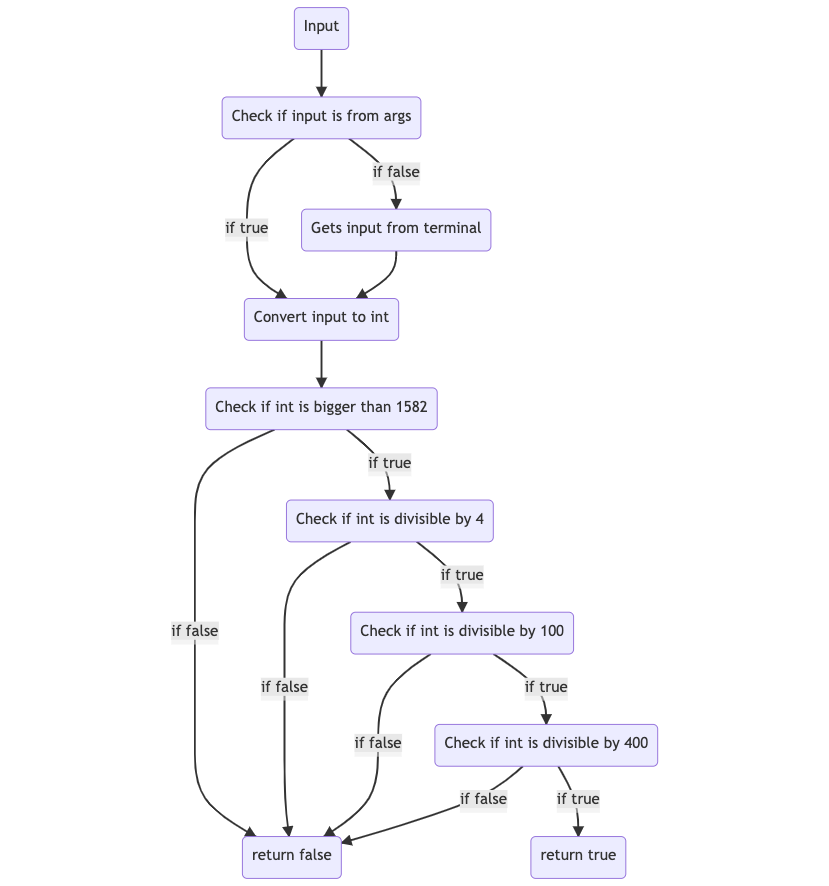
\includegraphics[width=0.9\textwidth, angle =-90 ]{mermaid-diagram-2022-09-06-114544.png}
\end{sidewaysfigure}

\end{document}
